\documentclass[border=10pt]{standalone}

\usepackage{tikz}
\usepackage{tikzsymbols}
\usetikzlibrary{calc,patterns,shapes.geometric}

\def\centerarc[#1](#2)(#3:#4:#5){\draw[#1] ($(#2)+({#5*cos(#3)},{#5*sin(#3)})$) arc (#3:#4:#5);}

\begin{document}
	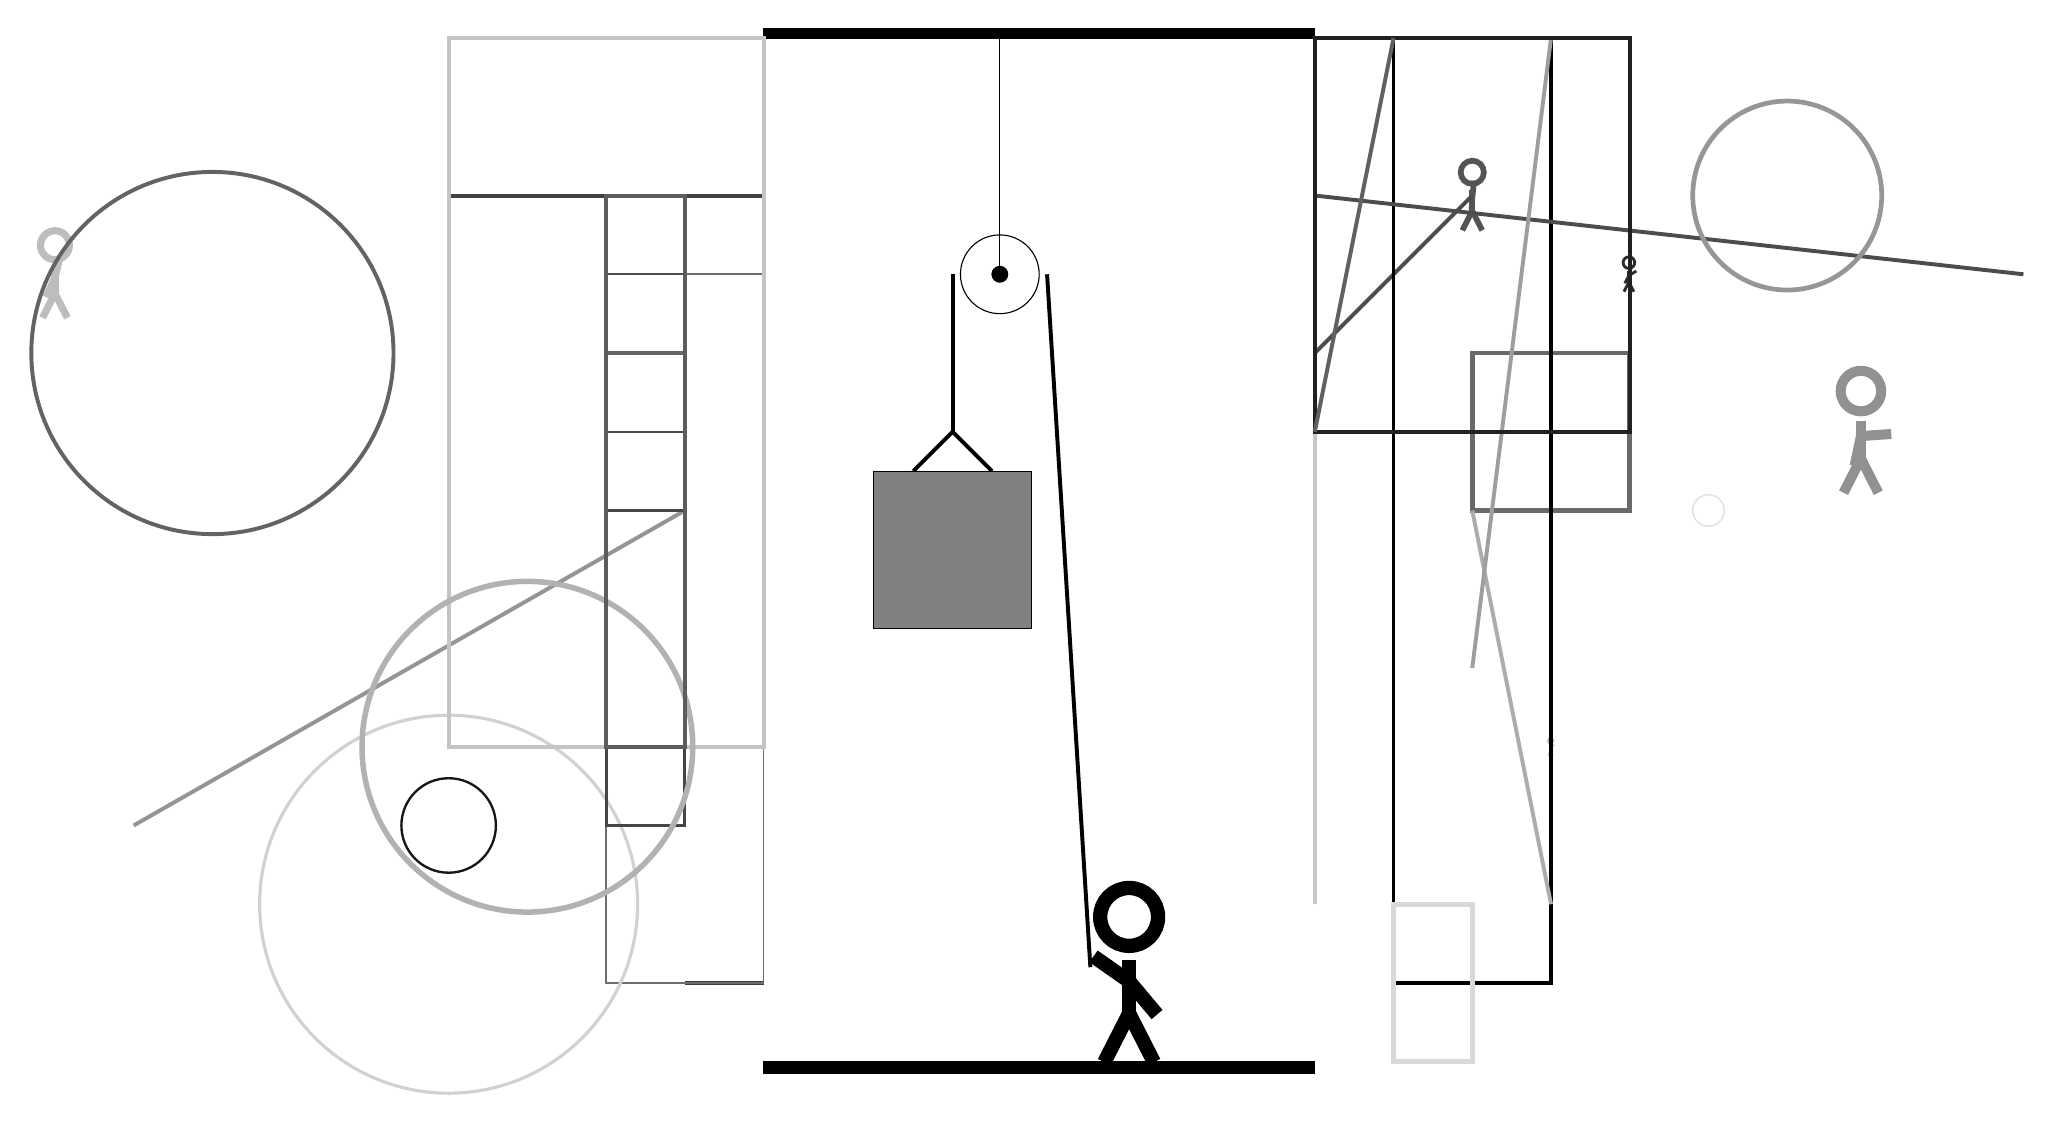
\begin{tikzpicture}
		%%%%% START %%%%%
		
		\draw[fill=black] (-2, 10) rectangle (5, 10.125);
		
		\draw (1, 7) circle (0.5);
		\draw[fill=black] (1, 7) circle (0.1);
		\draw (1, 10) -- (1, 7);
		
		\draw[line width=0.5mm] (-0.1, 4.5) -- (0.4, 5.0) -- (0.9, 4.5);
		\draw[fill=black!50] (-0.6, 4.5) rectangle (1.4, 2.5);
		
		\draw[line width=0.5mm] (0.4, 7) -- (0.4, 5.0);
		\centerarc[line width=0.5mm](1, 7)(0:180:0.6);
		\draw[line width=0.5mm](1.6, 7) -- (2.15, -1.8);
		
		\node[line width=0.7mm, color=black!27] at (8, 1) {\Strichmaxerl[1][82][35]};
		
		\draw[line width=0.6mm, color=black!59] (7, 4) rectangle (9, 6);
		\node[line width=0.3mm, color=black!67] at (7, 8) {\Strichmaxerl[4][87][84]};
		\draw[line width=0.3mm, color=black!47] (5, 6) rectangle (5, 9);
		\draw[line width=0.5mm, color=black!22] (5, -1) rectangle (5, 10);
		\draw[line width=0.5mm, color=black!76](-2, -2) -- (-3, -2);
		\draw[line width=0.5mm, color=black!60] (-4, 1) rectangle (-3, 6);
		\draw[line width=0.5mm, color=black!70](7, 8) -- (5, 6);
		\draw [line width=0.3mm, color=black!91](-6, 0) circle (0.6);
		\draw[line width=0.2mm, color=black!57] (-2, 7) rectangle (-4, -2);
		\draw [line width=0.4mm, color=black!18](-6, -1) circle (2.4);
		\draw[line width=0.4mm, color=black!100] (6, 10) rectangle (8, -2);
		\draw[line width=0.3mm, color=black!70] (-3, 7) rectangle (-4, 5);
		
		\node[line width=0.4mm, color=black!26] at (-11, 7) {\Strichmaxerl[5][66][76]};
		\draw[line width=0.5mm, color=black!74] (-2, 8) rectangle (-6, 8);
		\draw[line width=0.5mm, color=black!42](-3, 4) -- (-10, 0);
		\node[line width=0.3mm, color=black!83] at (9, 7) {\Strichmaxerl[2][62][31]};
		\draw[line width=0.5mm, color=black!32](8, -1) -- (7, 4);
		\draw[line width=0.5mm, color=black!70](5, 8) -- (14, 7);
		\node[line width=0.4mm, color=black!43] at (12, 5) {\Strichmaxerl[7][78][4]};
		\draw[line width=0.5mm, color=black!38](8, 10) -- (7, 2);
		
		\draw [line width=0.5mm, color=black!55](-9, 1) circle (0.0);
		\draw[line width=0.6mm, color=black!15] (7, -3) rectangle (6, -1);
		\draw[line width=0.5mm, color=black!87] (5, 10) rectangle (9, 5);
		\draw[line width=0.5mm, color=black!23] (-2, 10) rectangle (-6, 1);
		\draw[line width=0.4mm, color=black!73] (-4, 4) rectangle (-3, 0);
		\draw[line width=0.5mm, color=black!62](5, 5) -- (6, 10);
		\draw [line width=0.7mm, color=black!30](-5, 1) circle (2.1);
		
		\draw [line width=0.5mm, color=black!61](-9, 6) circle (2.3);
		\draw [line width=0.2mm, color=black!11](10, 4) circle (0.2);
		\draw[line width=0.5mm, color=black!64] (-4, 1) rectangle (-3, 8);
		
		\draw [line width=0.6mm, color=black!41](11, 8) circle (1.2);
		
		\node at (2.6, -1.9) {\Strichmaxerl[10][-35][-50]};
		
		\draw[fill=black] (-2, -3) rectangle (5, -3.15);
		
		%%%%% END %%%%%
	\end{tikzpicture}
\end{document}